\documentclass[aps,reprint]{revtex4-2}

\usepackage{microtype}
\usepackage{fix-cm} % Remove font size substitution warnings
\usepackage{amsmath} % must be loaded before newtxmath
\usepackage{amssymb}
\usepackage{amsthm}
\usepackage{siunitx}
\usepackage{physics}
\usepackage[mathic=true]{mathtools}
\usepackage{graphicx}
\usepackage[usenames,dvipsnames]{xcolor}
\usepackage{tikz}

\usepackage[semibold]{libertine} % a bit lighter than Times--no osf in math
\usepackage[libertine,vvarbb]{newtxmath}
\usepackage[scr=esstix,cal=boondoxo]{mathalfa}
\usepackage{bm} % load after all math to give access to bold math
\renewcommand\mathrm\textnormal%

% \allowdisplaybreaks%

\usepackage[pdfusetitle]{hyperref}
\hypersetup{%
  hypertexnames=false, % For compatibility with autonum
  colorlinks,
  allcolors=MidnightBlue,
  citecolor=OliveGreen,
}
\urlstyle{same}
\usepackage{autonum}

\theoremstyle{plain}
\newtheorem{thm}{Theorem}[section]
\newtheorem{lem}{Lemma}
\theoremstyle{definition}
\newtheorem{defn}{Definition}
\newtheorem{post}{Postulate}

\graphicspath{{figs/}}

\usepackage{minted}
\setmonofont[Scale=MatchLowercase]{Iosevka}
\setminted{%
  fontsize=\scriptsize,
  mathescape, style=friendly, baselinestretch=0.9, breaklines
}
\setminted[wolfram]{%
  style=mathematica
}

\renewcommand\leq\leqslant%
\renewcommand\geq\geqslant%

\renewcommand\phi\varphi%


\newcommand\im{\mathrm{i}\mkern1mu}
\renewcommand\ln{\operatorname{\mathrm{ln}}}
\renewcommand\lg{\operatorname{\mathrm{lg}}}
\renewcommand\log{\operatorname{\mathrm{log}}}
\renewcommand\exp{\operatorname{\mathrm{exp}}}
\renewcommand\tr{\operatorname{\mathrm{tr}}}
\renewcommand\det{\operatorname{\mathrm{det}}}

\newcommand\ZZ{\mathbb{Z}}
\newcommand\QQ{\mathbb{Q}}
\newcommand\CC{\mathbb{C}}
\newcommand\RR{\mathbb{R}}

\newcommand{\opr}[1]{\mathsf{#1}}%
\newcommand\idsopr{\mathbb{1}}
\newcommand\idopr{\opr{I}}
\newcommand\sopr\mathcal%
\newcommand\cat\mathsf%
\newcommand\herm{\operatorname{\mathrm{He}}}

% \newcommand\lprod[2]{{\qty(#1,#2)}}
\newcommand\lprod\ip%

\newcommand\hilb{\mathcal{H}}
\newcommand\liou{\mathcal{L}}
\newcommand\ham{\opr{H}}
\newcommand\dop{\opr{ρ}}
\newcommand\tprod\otimes%

\newcommand\ensavg[2][\dop]{\ev{#2}_{\mkern-1.5mu{#1}}}%
\newcommand\sensavg[2][\dop]{\ev*{#2}_{\mkern-1.5mu{#1}}}%

\begin{document}
\title{Rensselaer \textsc{nsf} \textsc{reu} midterm report:\\
Quantifying visual information}
\author{Alex Striff}
\affiliation{Department of Physics, Reed College, Portland \textsc{or} 97202, \textsc{usa}}
\author{Vincent Meunier}
\affiliation{Department of Physics, Applied Physics, and Astronomy, Rensselaer
Polytechnic Institute, Troy \textsc{ny} 12180, \textsc{usa}}
\date{July 10, 2020}
\begin{abstract}
  We attribute a notion of lost information (entropy) to digital images based on
  considering pixel value fluctuations that are considered imperceptible or
  irrelevant to understanding the content of an image. This information is
  precisely defined in the framework of information theory, and is influenced by
  an analogous situation in statistical physics. Using this analogy enables us
  to compute the entropy using the Wang-Landau algorithm for the density of
  states developed for use in statistical physics. Given the results, we discuss
  potential extensions of the model that better resemble the known physical and
  biological processes that take place in the visual system.
\end{abstract}
\maketitle

\section{Introduction}

The human visual system is crucial for survival. While this system gathers
useful information from our environment, it remains imperfect. A precise
understanding of the information lost in sensation may guide future
understanding of the information we do gather, as well as inform the design of
image compression and reconstruction algorithms for human consumption.

As a simple model for this lossy process, we consider slightly varying the pixel
values of a grayscale image to produce different images that are not percieved
to be different, or that are not different enough to change the qualitative
impression of the image on an observer. The freedom to choose different modified
images represents information that is lost. What follows is a description of how
we can quantify this information, and then how we can calculate it for
particular images.

\section{Theory}

\subsection{Information Theory}\label{sec:information-theory}

A mathematical notion of information is provided by the work of
Shannon~\cite{shannon1948mathematical}. In the view of classical information
theory, \emph{information} is a property of an event, in the sense of a random
process. To this end, we consider a random variable $X$ with support
$\mathcal{X}$ and probabilities $p(x)$ for $x \in \mathcal{X}$. As regards
communication, the information $I(x)$ required to describe the event $X = x$
should satisfy intuitive axioms:
\begin{itemize}
  \item If $p(x) = 1$, the event is certain to happen and no information is
    required to describe its occurence: $I(x) = 0$.
  \item If $p(x) < p(x')$, then $x$ is less likely to happen, and ought to
    require more information to describe: $I(x) > I(x') \geq 0$. As an analogy,
    compare the phrases ``nightly'' and ``once in a full moon:'' The less
    probable event has a longer description.
  \item For independent events $x$ and $y$, it makes no difference to describe
    the combined event $(x,\, y)$ instead of each event individually: $I(x,\, y)
    = I(x) + I(y)$.
\end{itemize}

Given these axioms, the only solution is the
\emph{self-information}~(Theorem~\ref{thm:self-information})
\begin{equation}
  I(x)
  = -\log p(x),
  \label{eq:self-information}
\end{equation}
where the base of the logarithm determines the units of information: base two
($\lg$) gives \emph{bits} and base $e$ ($\ln$) gives \emph{nats}. The
information of the entire random variable may then be defined as the average
of~\eqref{eq:self-information} over all events, which is known as the
\emph{Shannon entropy}
\begin{equation}
  H
  = -\sum_{x \in \mathcal{X}} p(x) \log p(x).
  \label{eq:shannon-entropy}
\end{equation}
The Shannon entropy may also be derived from intuitive axioms similar to those
for the self information~\cite{shannon1948mathematical,jaynes1957information}.

\subsection{The maximum entropy principle (\textsc{MaxEnt})}\label{sec:maxent}

A physicist familiar with statistical mechanics might wonder why Shannon's
entropy~\eqref{eq:shannon-entropy} has the same mathematical form as the
thermodynamic state variable for temperature
\begin{equation}
  S
  = -k_B \sum_{x \in \mathcal{X}} p(x) \ln p(x),
  \label{eq:gibbs-entropy}
\end{equation}
which we may call the \emph{Gibbs entropy}. This connection between information
theory and statistical physics was developed by Jaynes, culminating in the
maximum entropy principle (\textsc{MaxEnt})~\cite{jaynes1957information}. We
would like to make predictions about systems given some macroscopic quantities
that we observe. To do so, we must assign probabilities to microstates, which we
ought to do in an unbiased way, subject to the constraints that average
macroscopic quantities take their observed values. Jaynes argues that this
unbiased assignment corresponds to maximizing the entropy, and describes how
this subjective assignment can be expected to make physical predictions, while
an objective assignment of probabilities is required to understand the
microscopic mechanisms behind these predictions. In particular, maximizing the
entropy with constrained average energy produces the canonical
distribution~\cite{jaynes1957information}
\[
  p(x)
  = \frac{1}{Z}e^{-\beta E(x)},
\]
where $\beta = \flatfrac{1}{k_B T}$ and the \emph{partition function} is
\[
  Z
  = \sum_{x \in \mathcal{X}} e^{-\beta E(x)},
\]
with the variates $x$ being different states of a system.

\subsection{Image fluctuations}

\begin{figure}
  \centering
  \tikzstyle{emph} = [fill=MidnightBlue]
  \begin{tikzpicture}[scale=0.5]%, every node/.style={transform shape}]
    \node[left] at (1.25*1, 1 + 0.5) {\small$1$};
    \node[left] at (1.25*1, 5 + 0.5) {\small$M$};
    \node[below] at (1.25*1 + 0.5,1) {\small$1$};
    \node[below] at (1.25*4 + 0.5,1) {\small$N$};
    \fill[gray] (1.25*1,4) rectangle ++(1,1);
    \fill[emph] (1.25*1,3) rectangle ++(1,1);
    \fill[gray] (1.25*2,1) rectangle ++(1,1);
    \fill[emph] (1.25*2,5) rectangle ++(1,1);
    \fill[gray] (1.25*4,2) rectangle ++(1,1);
    \fill[emph] (1.25*4,4) rectangle ++(1,1);
    \draw[emph] (1.25*4 + 1, 2 + 0.5) -- ++(0.75,0);
    \draw[emph] (1.25*4 + 1, 4 + 0.5) -- ++(0.75,0);
    \draw[emph,<->,thick] (1.25*4 + 1.5, 2 + 0.5) -- ++(0,2)
      node[midway,right]{$\Delta E_N = 2$};
    \node (ellipses) at (1.25*3 + 0.5, 3 + 0.5) {$\cdots$};
    \foreach \x in {1,2,4} {%
      \foreach \y in {1,...,5} {%
        \draw (1.25*\x,\y) rectangle ++(1,1);
      }
    }
  \end{tikzpicture}
  \caption{The energy difference between base image pixel values
    (\textcolor{gray}{$\blacksquare$}) and modified image pixel values
    (\textcolor{MidnightBlue}{$\blacksquare$}).
  }\label{fig:image-levels}
\end{figure}

Given a base image $A$ with $N$ pixels which take integer gray values $1 \leq
a_i \leq M$, we define the \emph{energy} of a different image $B$ with gray
values $1 \leq b_i \leq M$ as
\[
  E_A(B)
  = \sum_{i=1}^N \abs{a_i - b_i},
\]
as depicted in Fig.~\ref{fig:image-levels}.

We would like to consider all possible modified images, but focus on images with
a typical value for the energy which indicates the size of fluctuations we are
considering. We do this by assigning a probability distribution to the images
with constrained average energy. Given the results of Sec.~\ref{sec:maxent}, we
choose the \textsc{MaxEnt} distribution, which we may consider as a canonical
ensemble. By thinking of our images as a physical system, we may apply tools
from statistical mechanics. We would like to know the entropy of the
\textsc{MaxEnt} distribution, which we will compute with the partition function as
\begin{equation}
  \flatfrac{S}{k_B}
  = \beta E + \ln Z.
  \label{eq:canonical-entropy}
\end{equation}
In turn, we obtain the partition function
\begin{equation}
  Z
  = \sum_{E \in E(\mathcal{X})} g(E) e^{-\beta E}
  \label{eq:partition-function}
\end{equation}
from the number of states $g(E)$ with energy $E$ (the \emph{density of states}).
For the case where the base image is all black ($a_i = 0$) or all white ($a_i =
M$), we may explicitly count that the density of states
is~(Theorem~\ref{thm:bw-g})
\begin{equation}
  g(E)
  = \sum_k {(-1)}^k \binom{N}{k} \binom{N + E - Mk - 1}{E - Mk}.
  \label{eq:bw-g}
\end{equation}
However, the situation for general grayscale images becomes more complicated.
For this reason and the ability to analyze more complex systems, we determine
the density of states numerically using the Wang-Landau
algorithm~\cite{wanglandau}.

\section{Methods}

The Wang-Landau algorithm (WL) was implemented to determine the density of
states for grayscale image fluctuations. Our implementation adapts the algorithm
described by Wang, Landau, et al.\ in~\cite{wanglandau,wanglandau-ajp} for
lattice models to work on the image fluctuation model we have described
(Appendix~\ref{sec:wanglandau-core}). The offset of the log density of states
was set by ensuring that the number of states from $\sum_E g(E)$ gave the total
number of states $M^N$. We then computed the entropy from the numerical density
of states with~\eqref{eq:canonical-entropy}.

\section{Results}

\begin{figure}
  \centering
  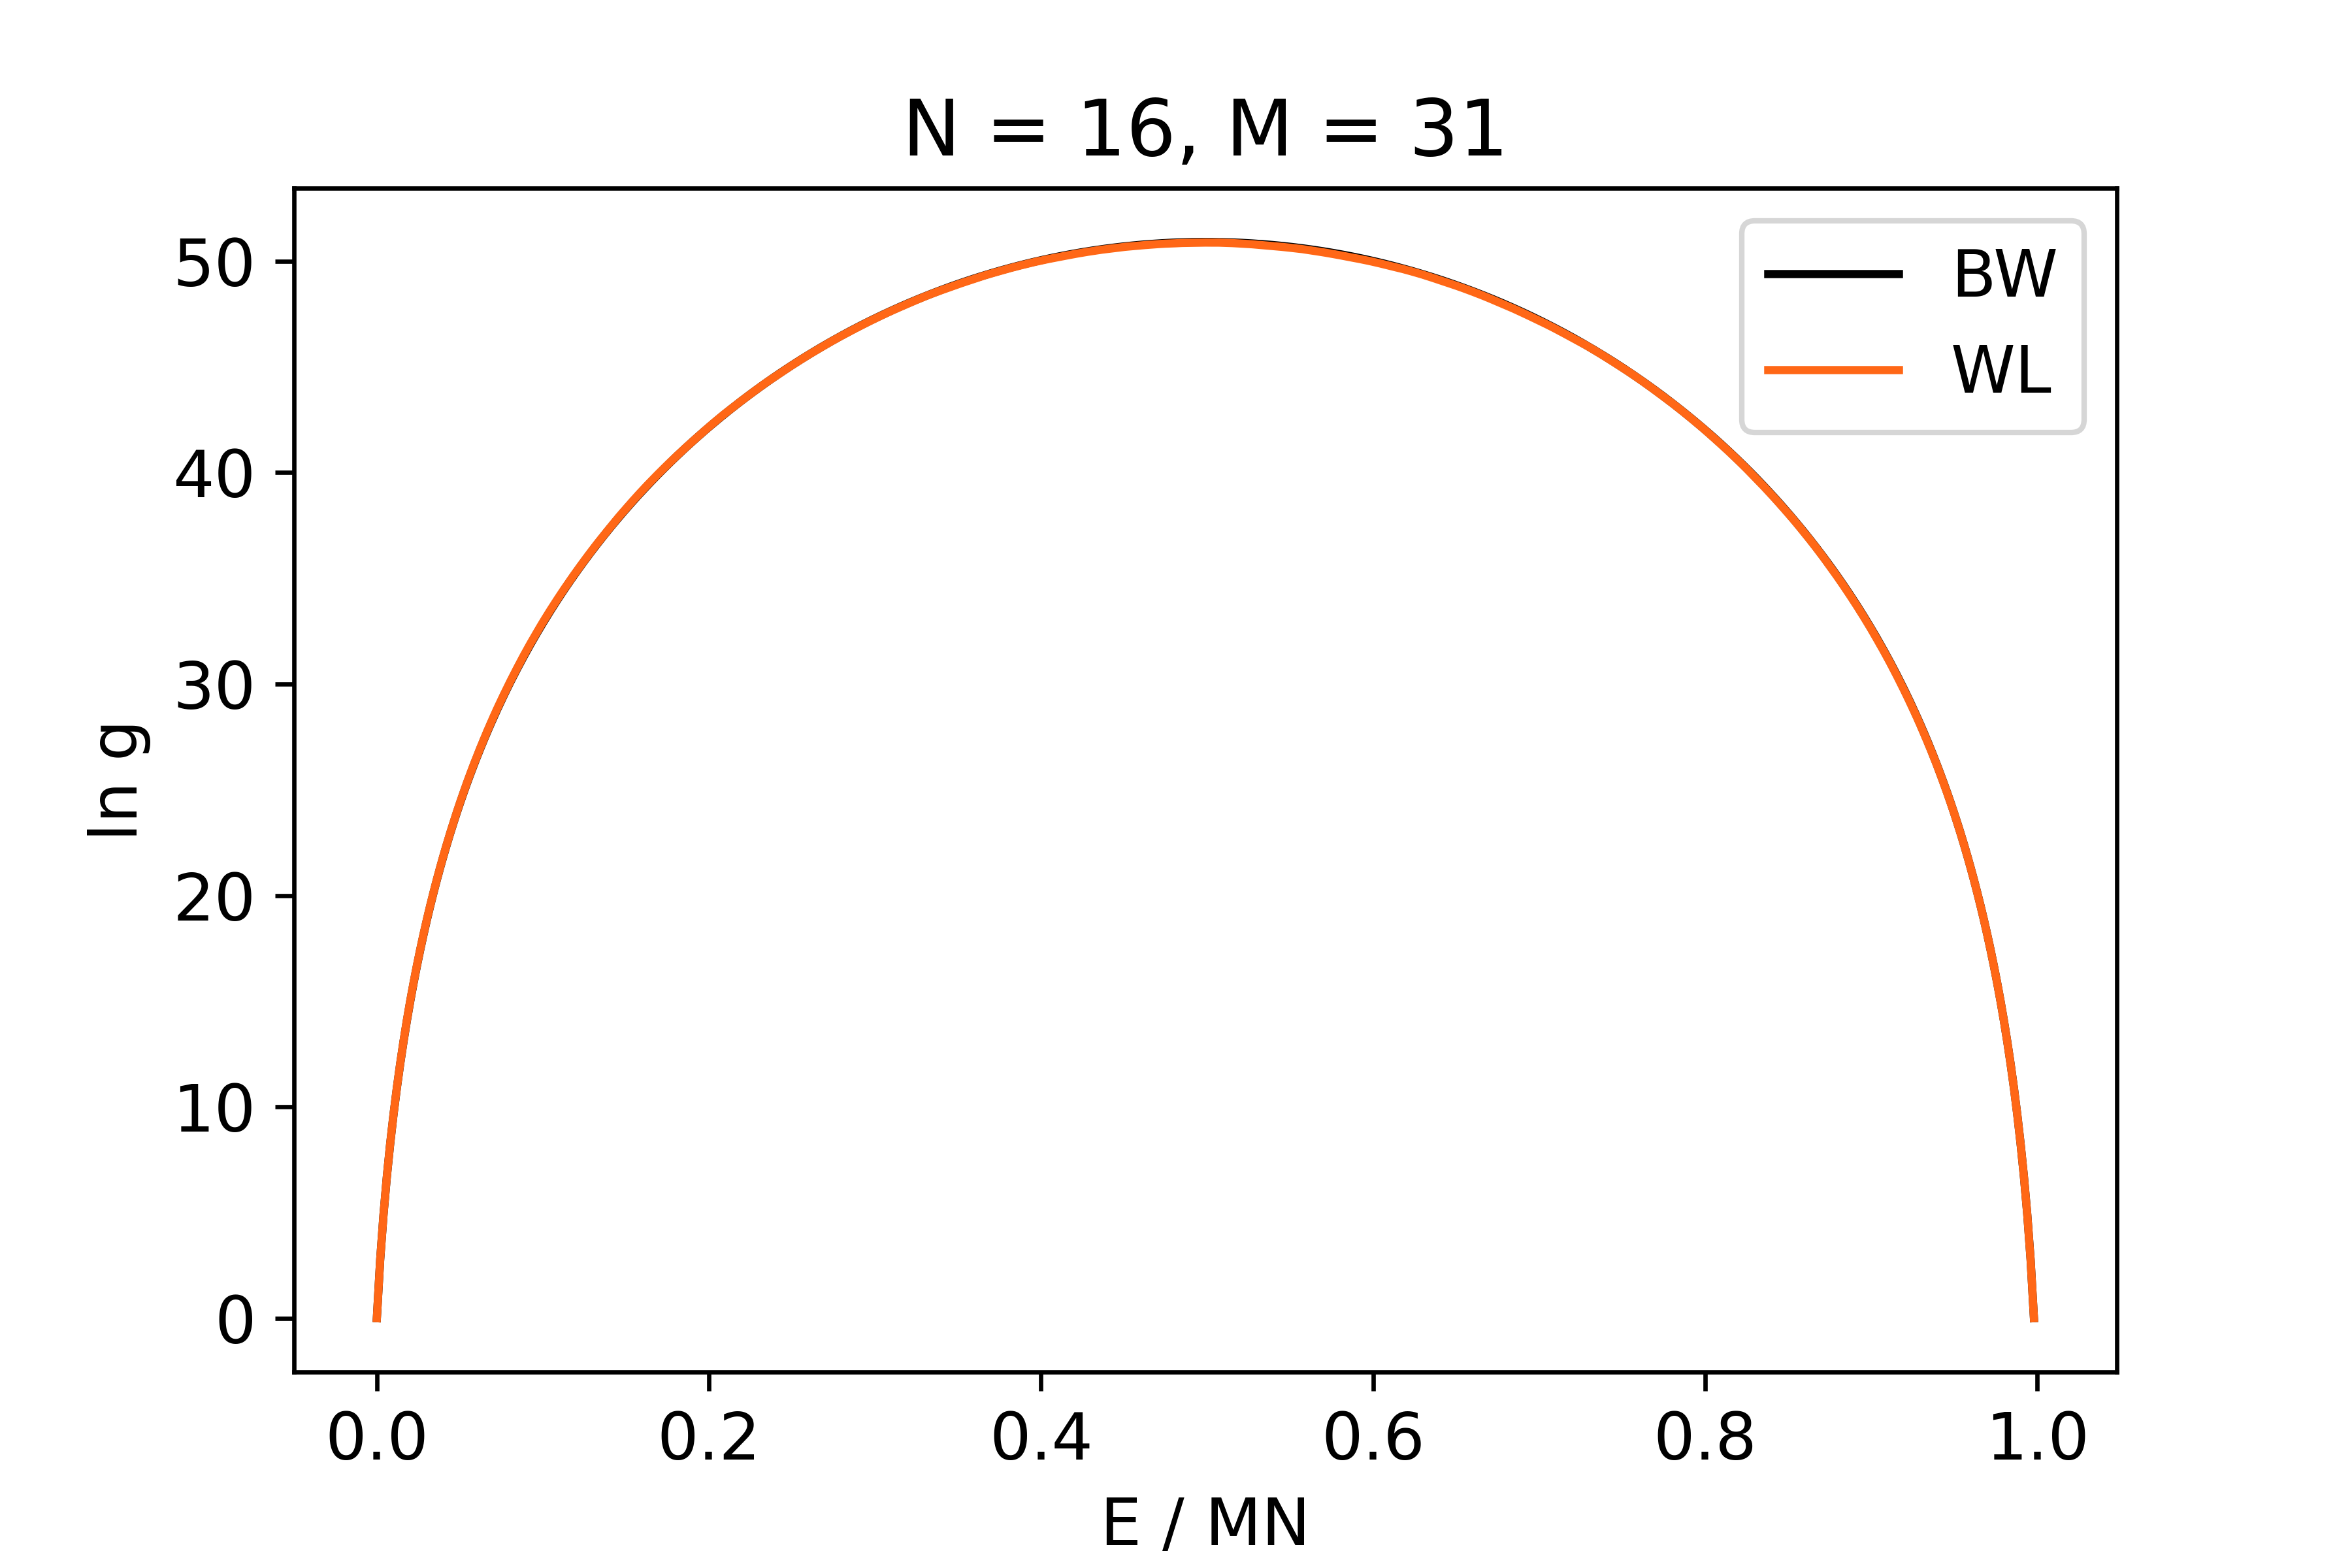
\includegraphics[width=\linewidth]{wanglandau-bw}
  \caption{The log density of states for a black image from the Wang-Landau
    algorithm (WL), compared to the exact result (BW). The two densities of
  states are indistinguishable.}\label{fig:wl-bw}
\end{figure}

\begin{figure}
  \centering
  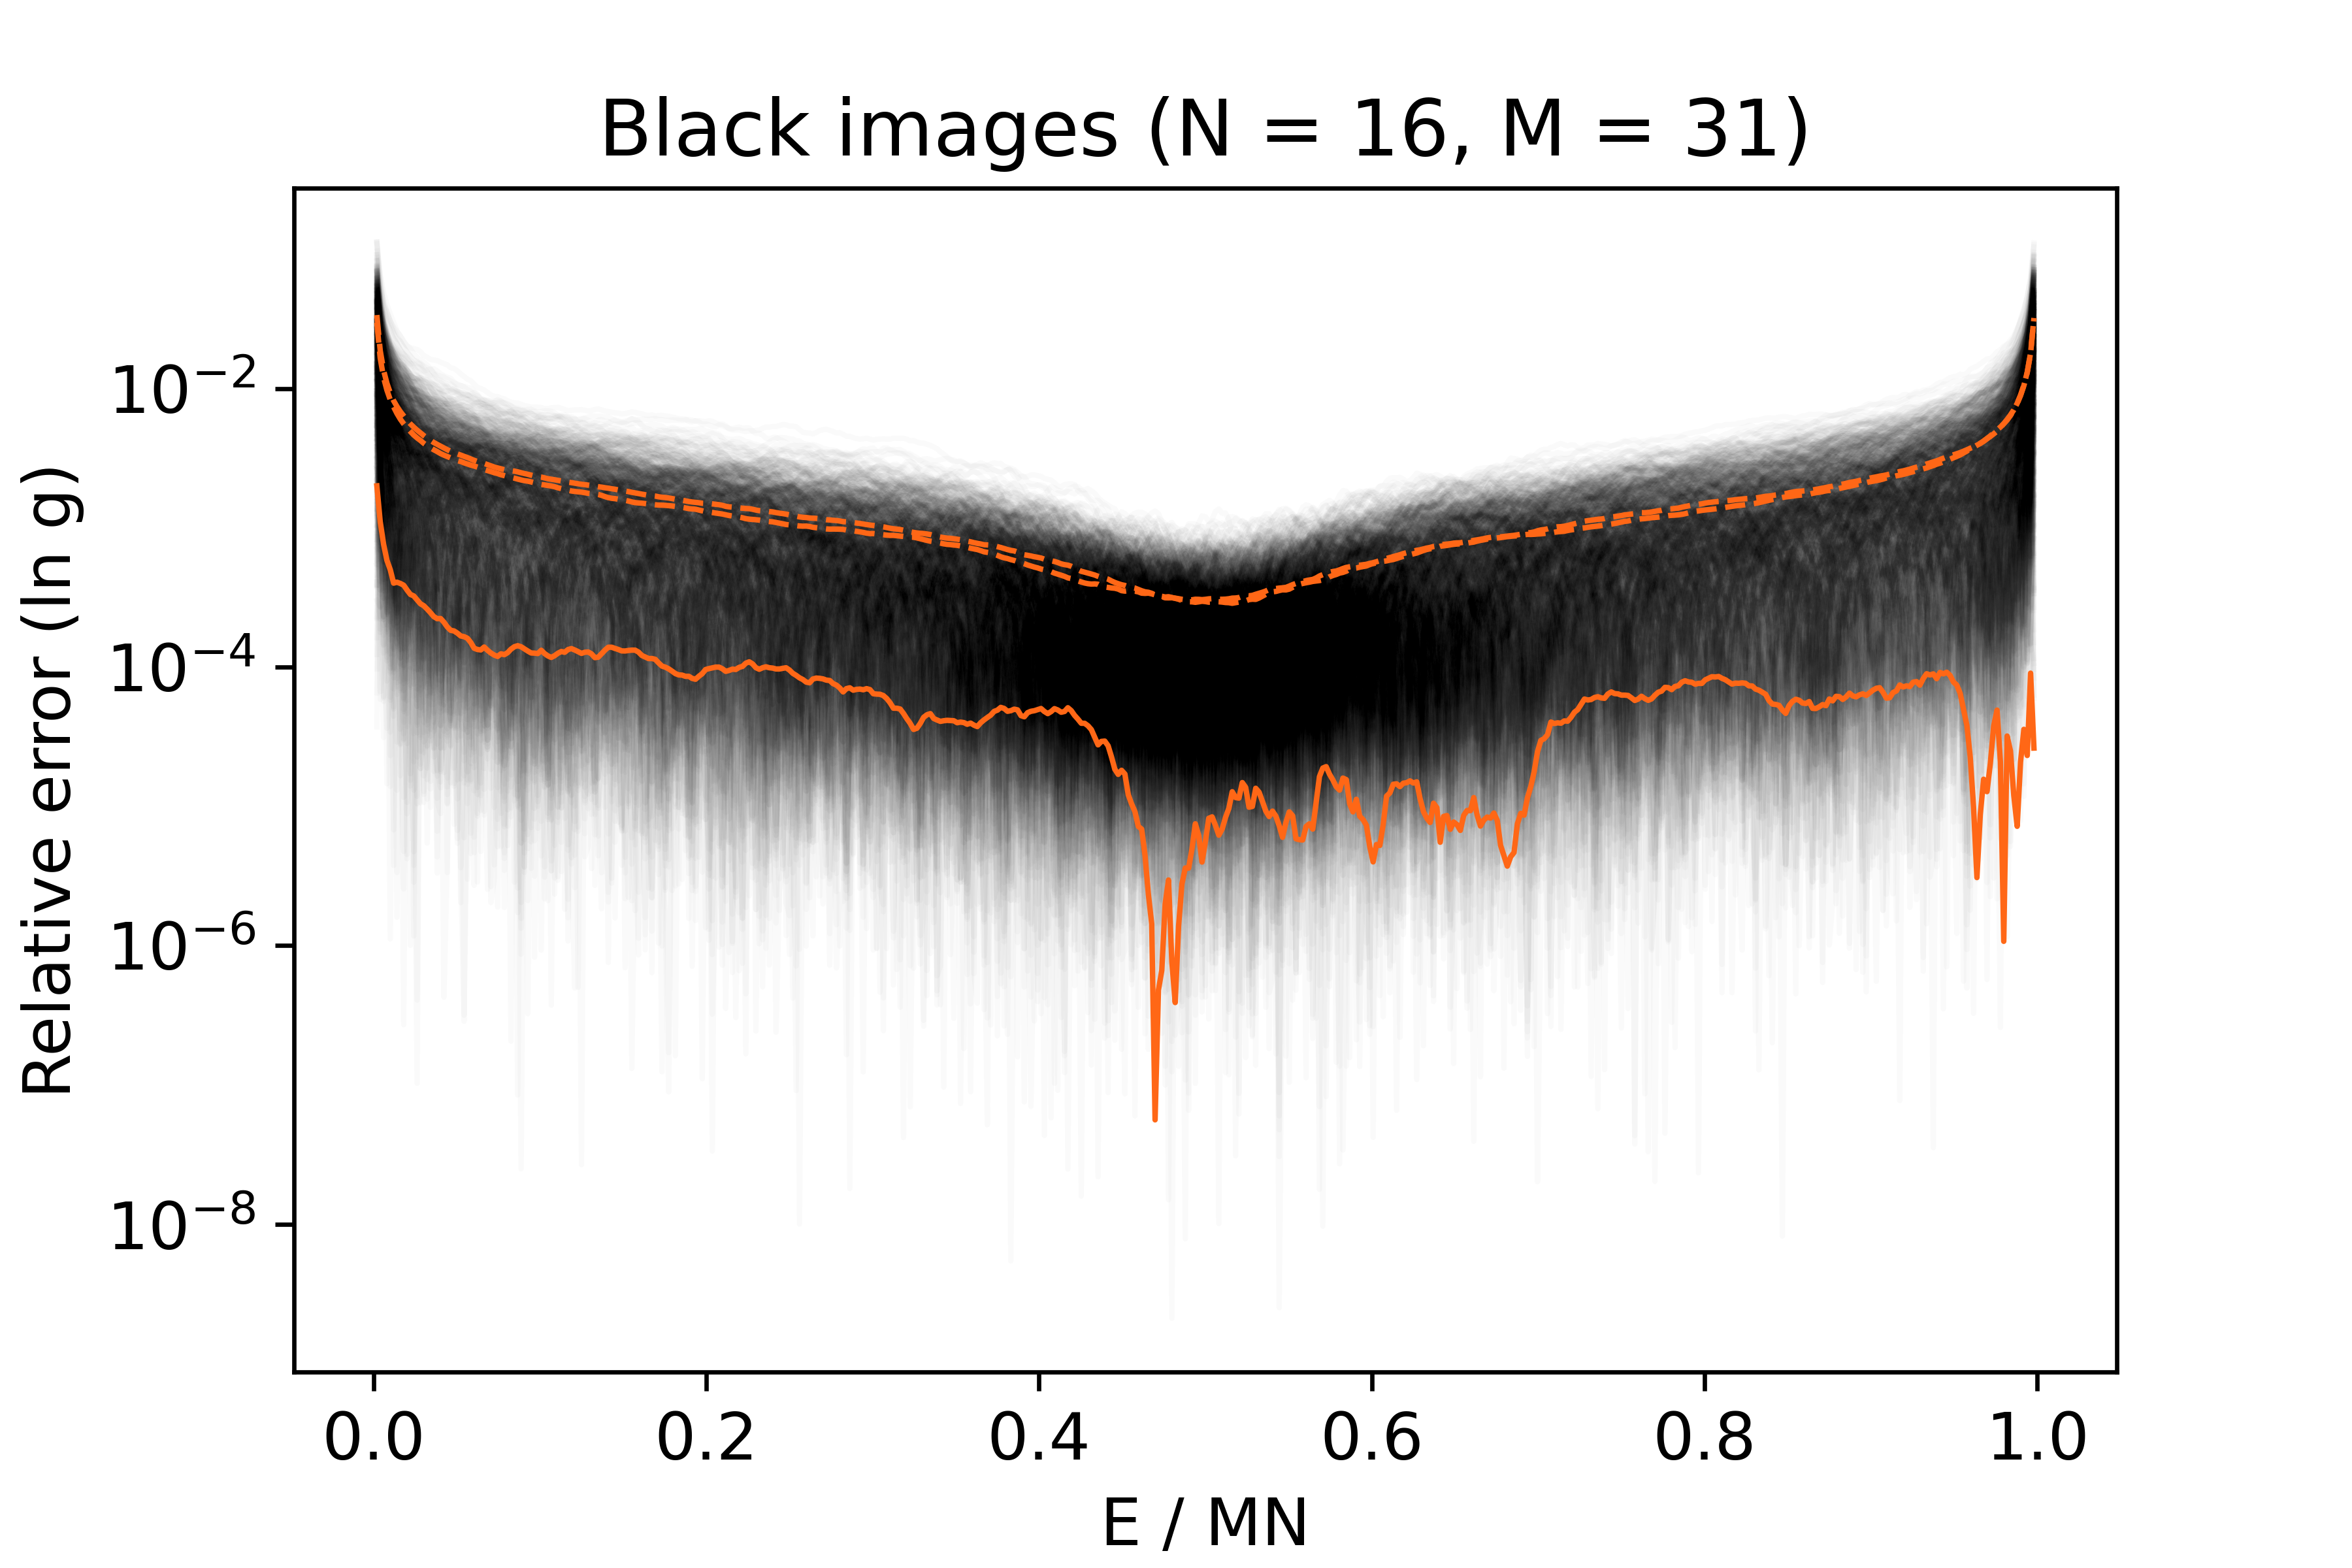
\includegraphics[width=\linewidth]{wanglandau-bw-relerror}
  \caption{The relative error in the log density of states for \num{1024} black
    image Wang-Landau simulations. The mean density of states is indicated
    in orange and the composite densities of states one standard deviation away
  are dashed.}\label{fig:wl-bw-relerror}
\end{figure}

\begin{figure}
  \centering
  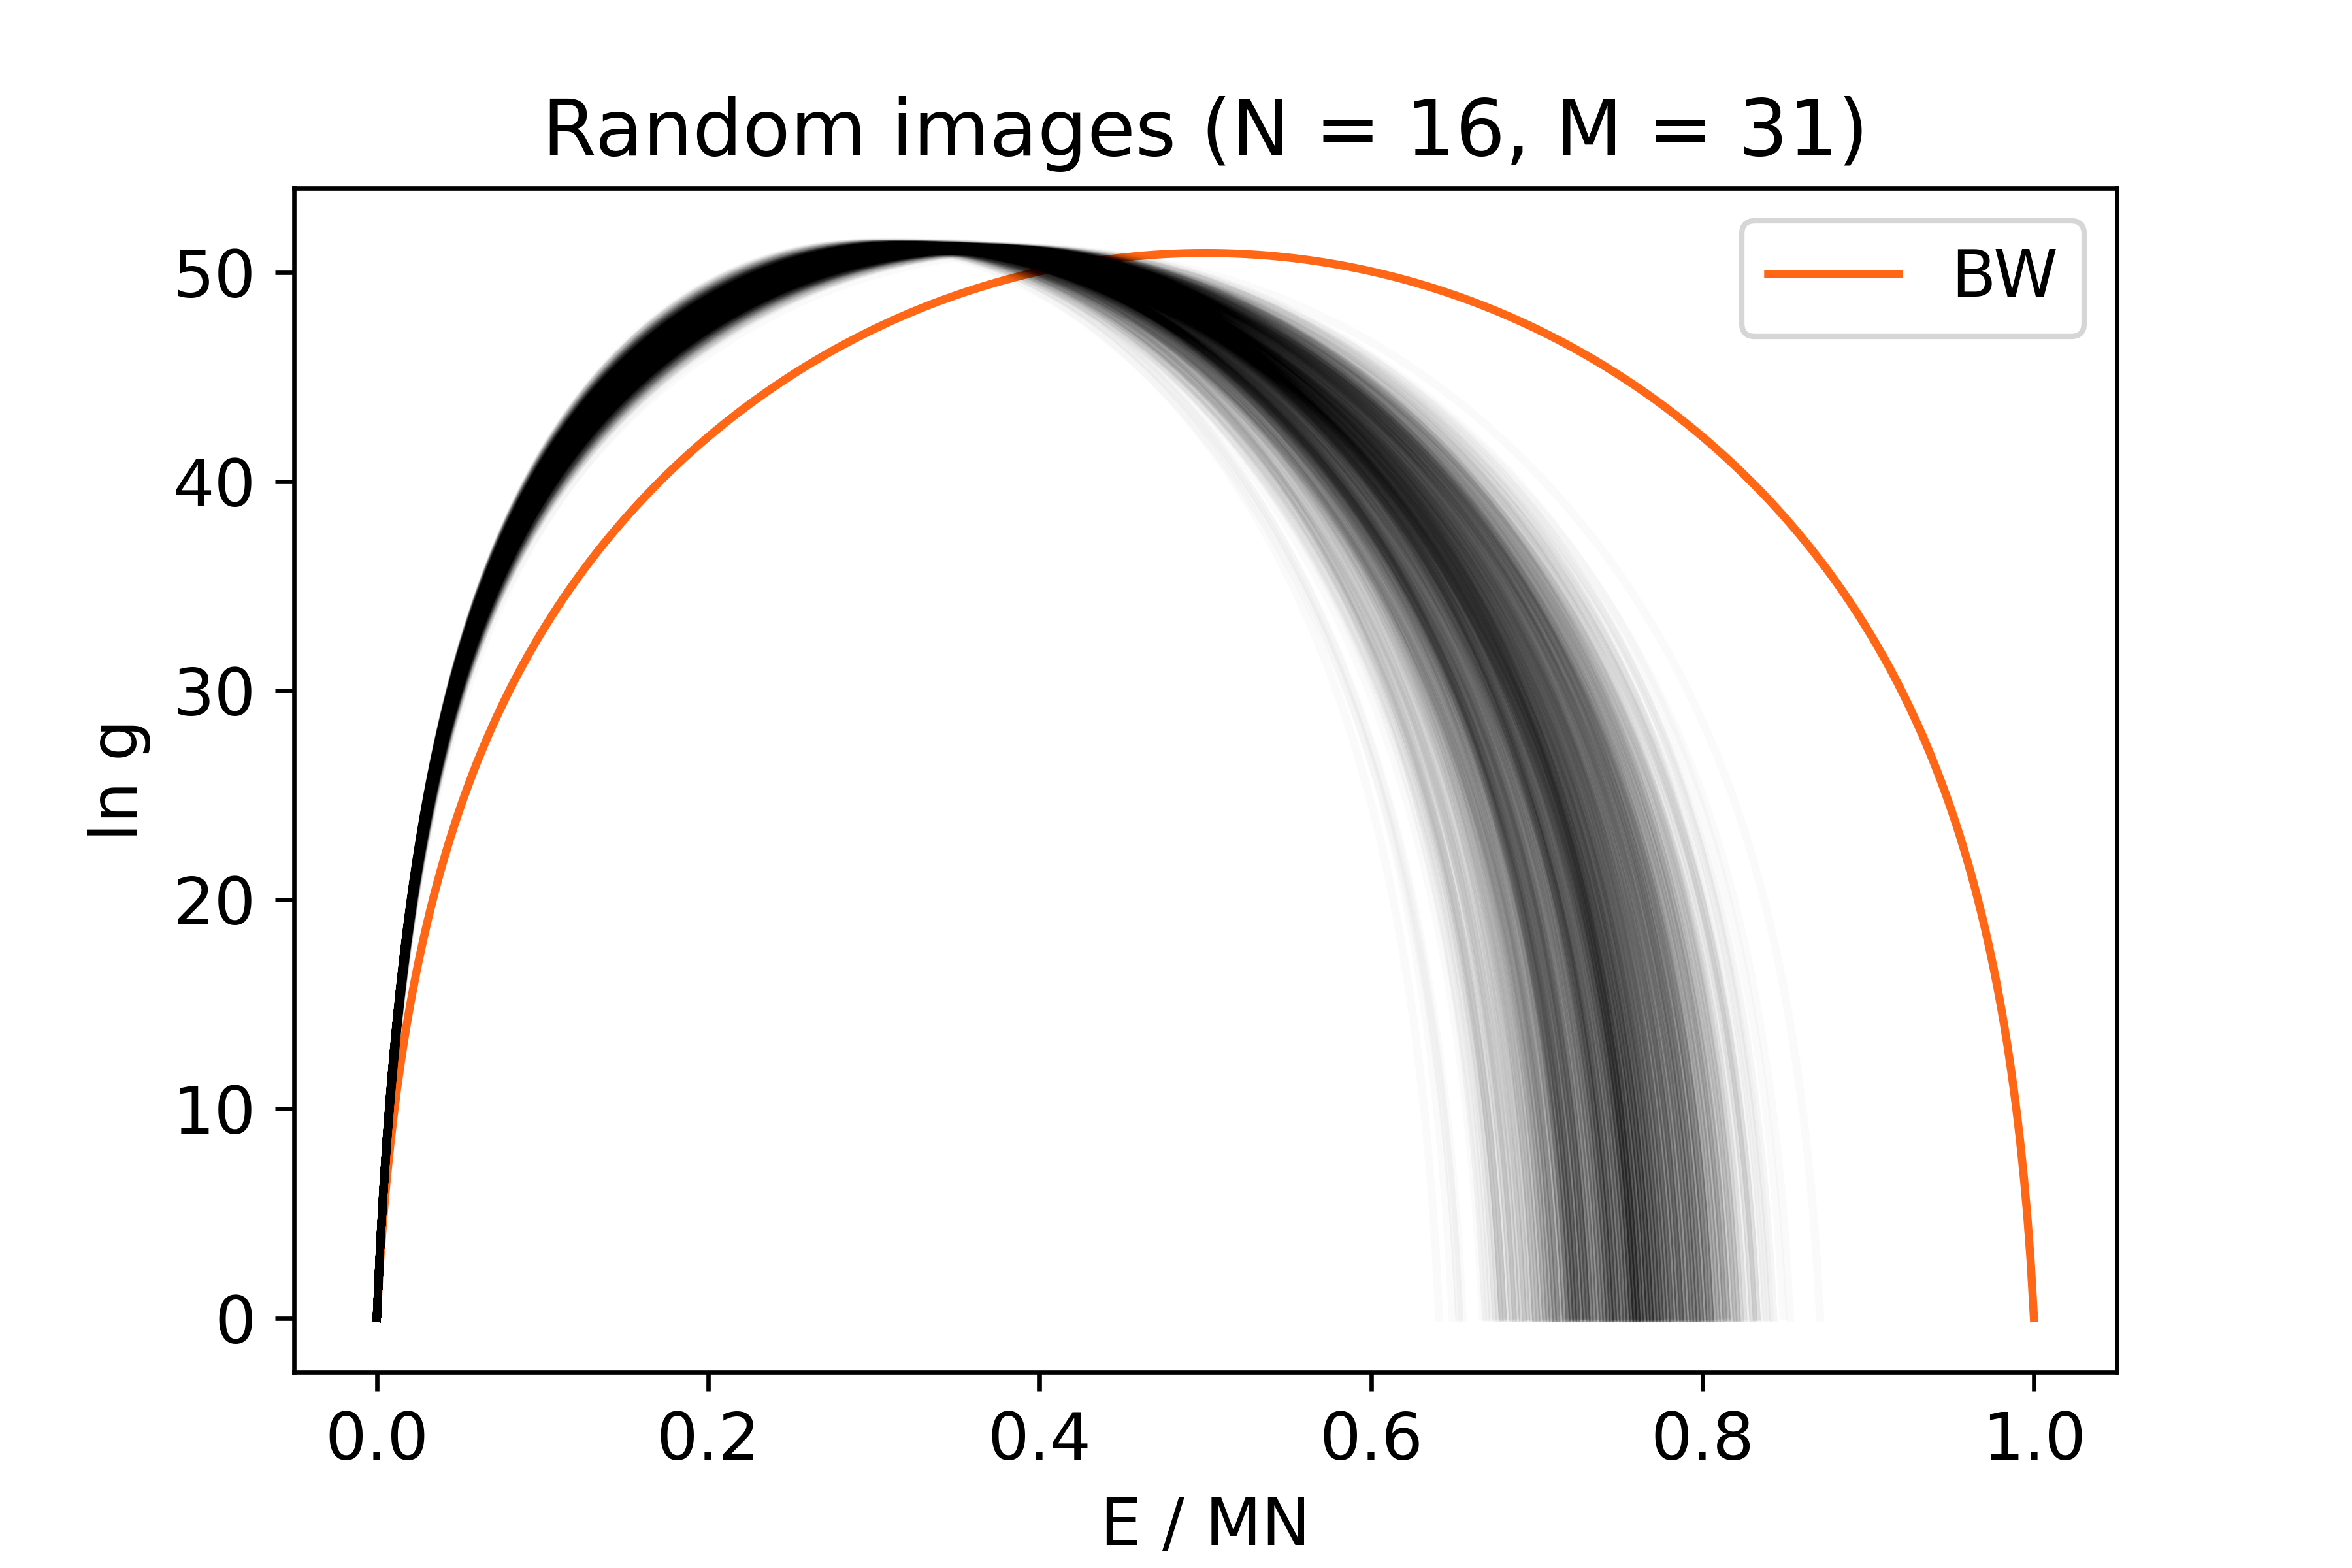
\includegraphics[width=\linewidth]{wanglandau-gray}
  \caption{The log density of states for \num{1024} random grayscale image
    Wang-Landau simulations. The black image result is provided as
  reference in orange (BW).}\label{fig:wl-gray}
\end{figure}

\begin{figure}
  \centering
  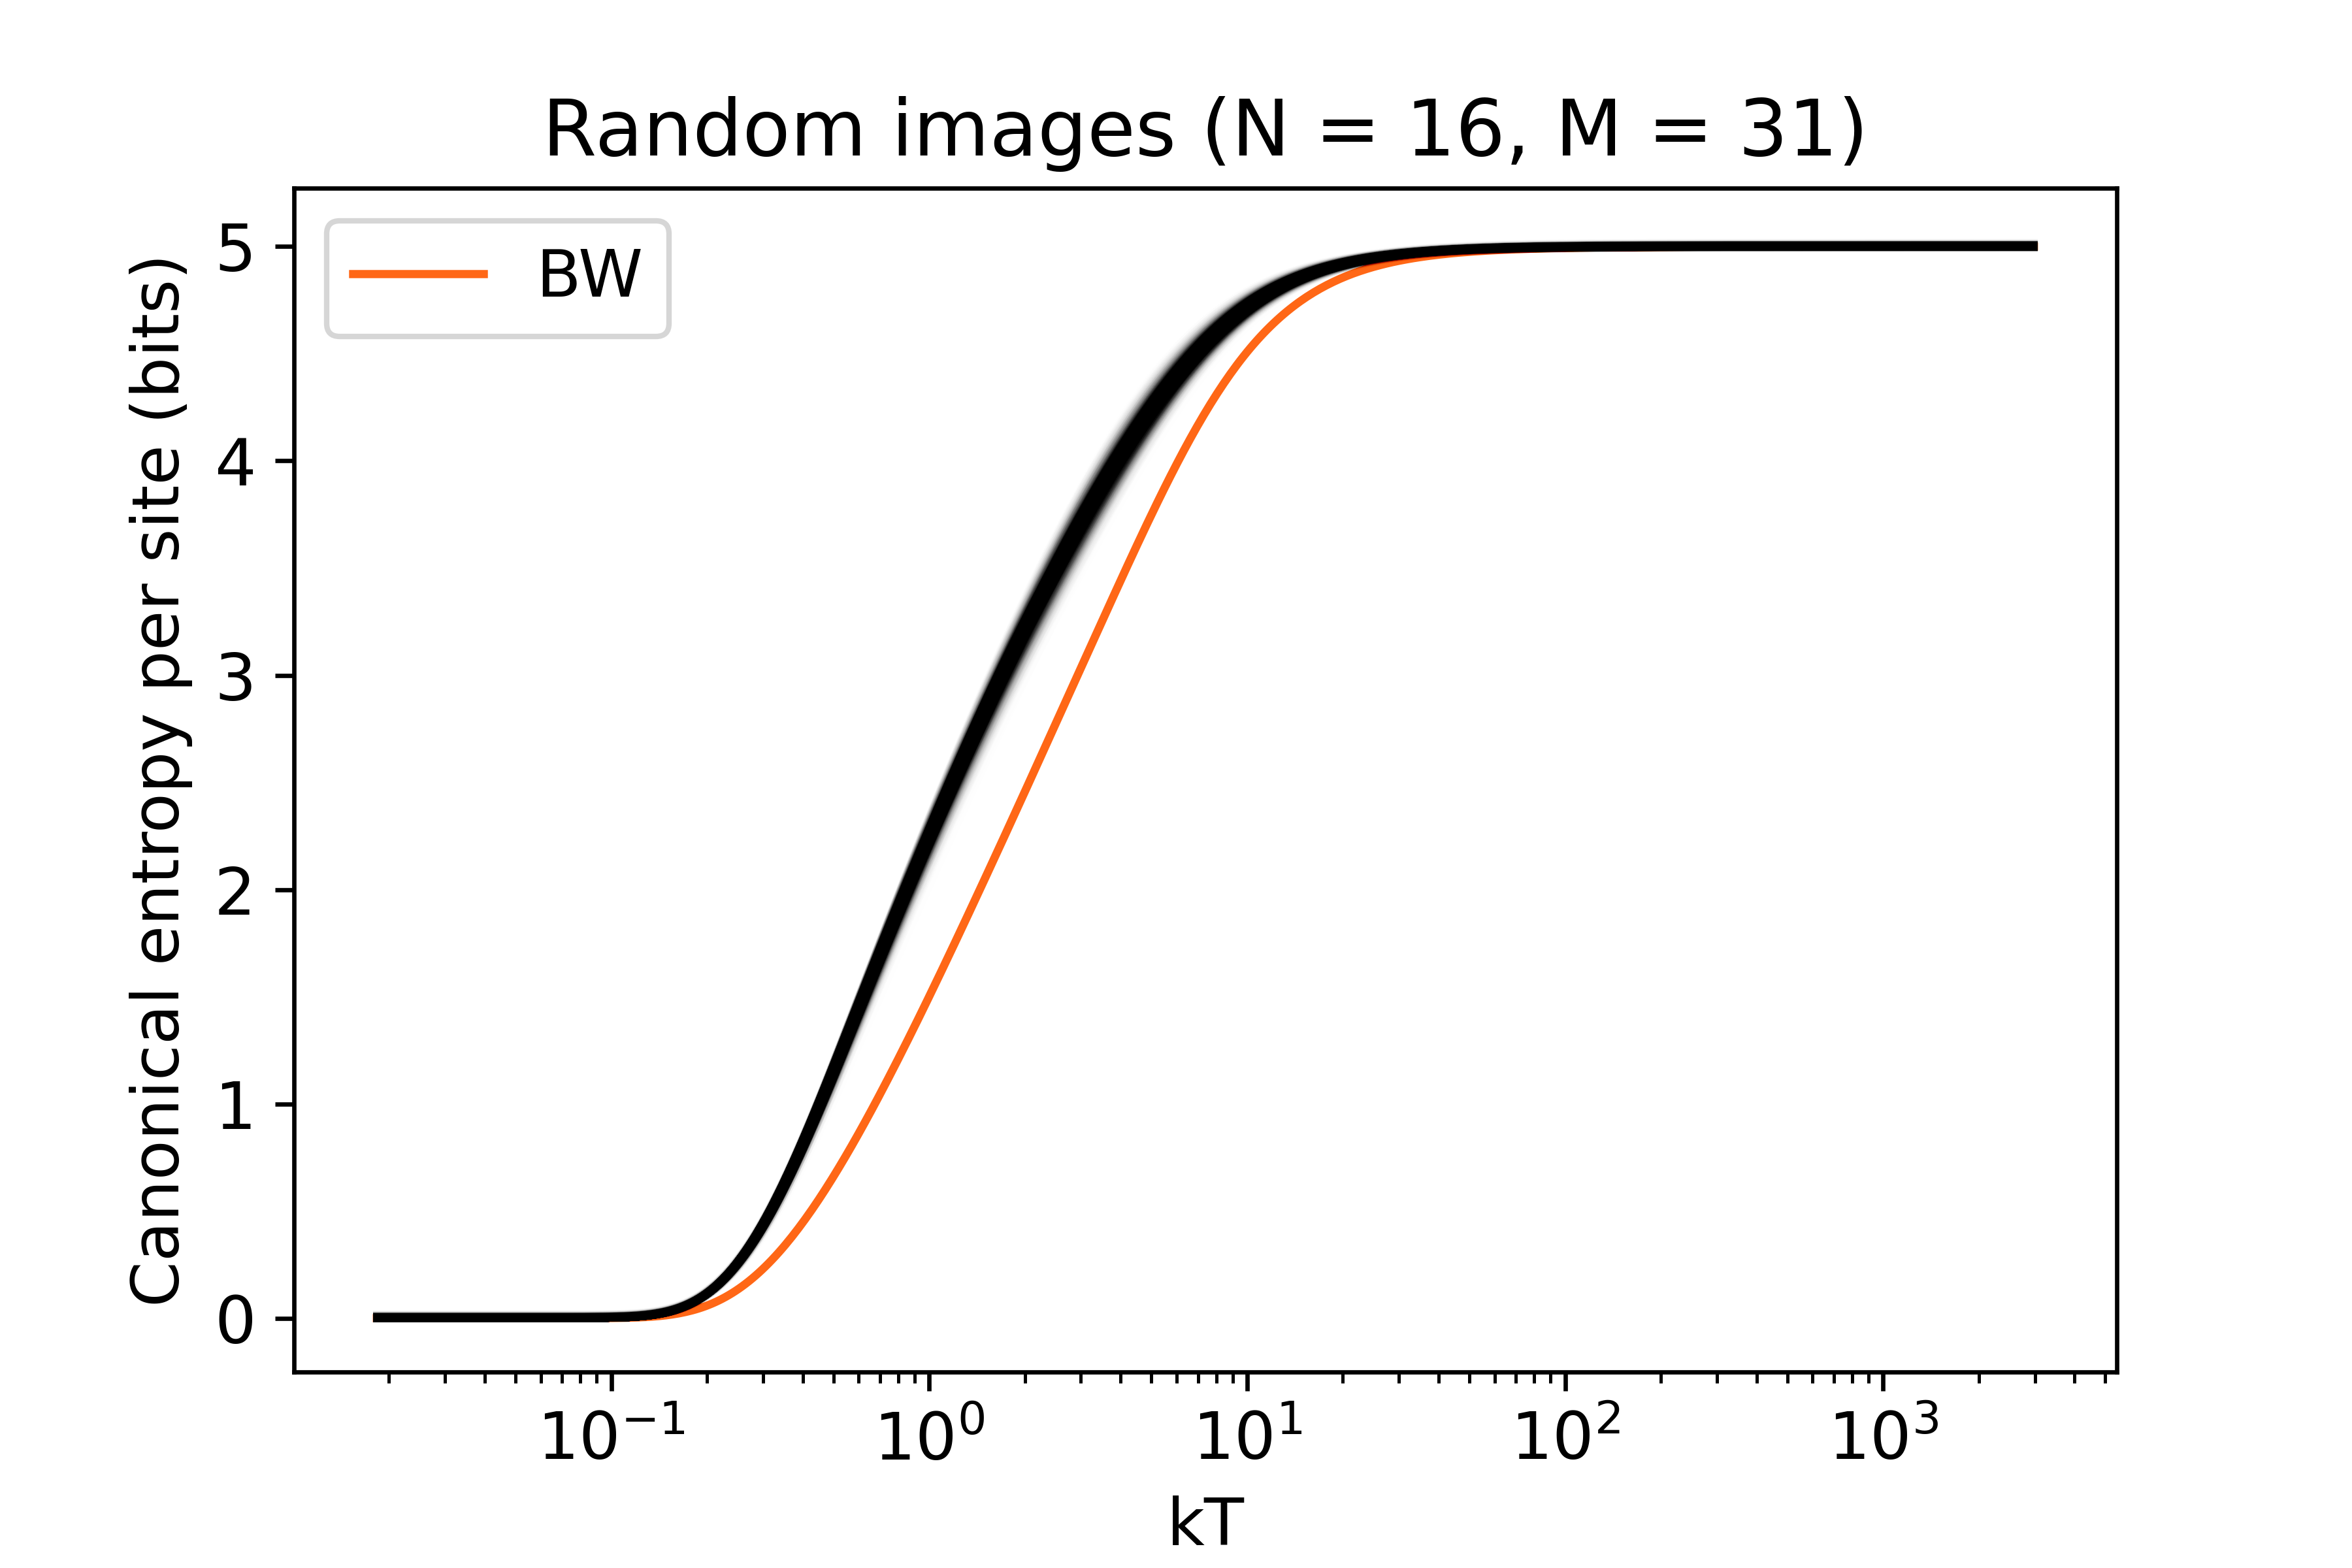
\includegraphics[width=\linewidth]{wanglandau-gray-S}
  \caption{The canonical entropy computed from the simulation density of states for
    \num{1024} random grayscale images. The entropy from the exact result for a
  black image is shown in orange (BW).}\label{fig:wl-gray-S}
\end{figure}

\begin{figure}
  \centering
  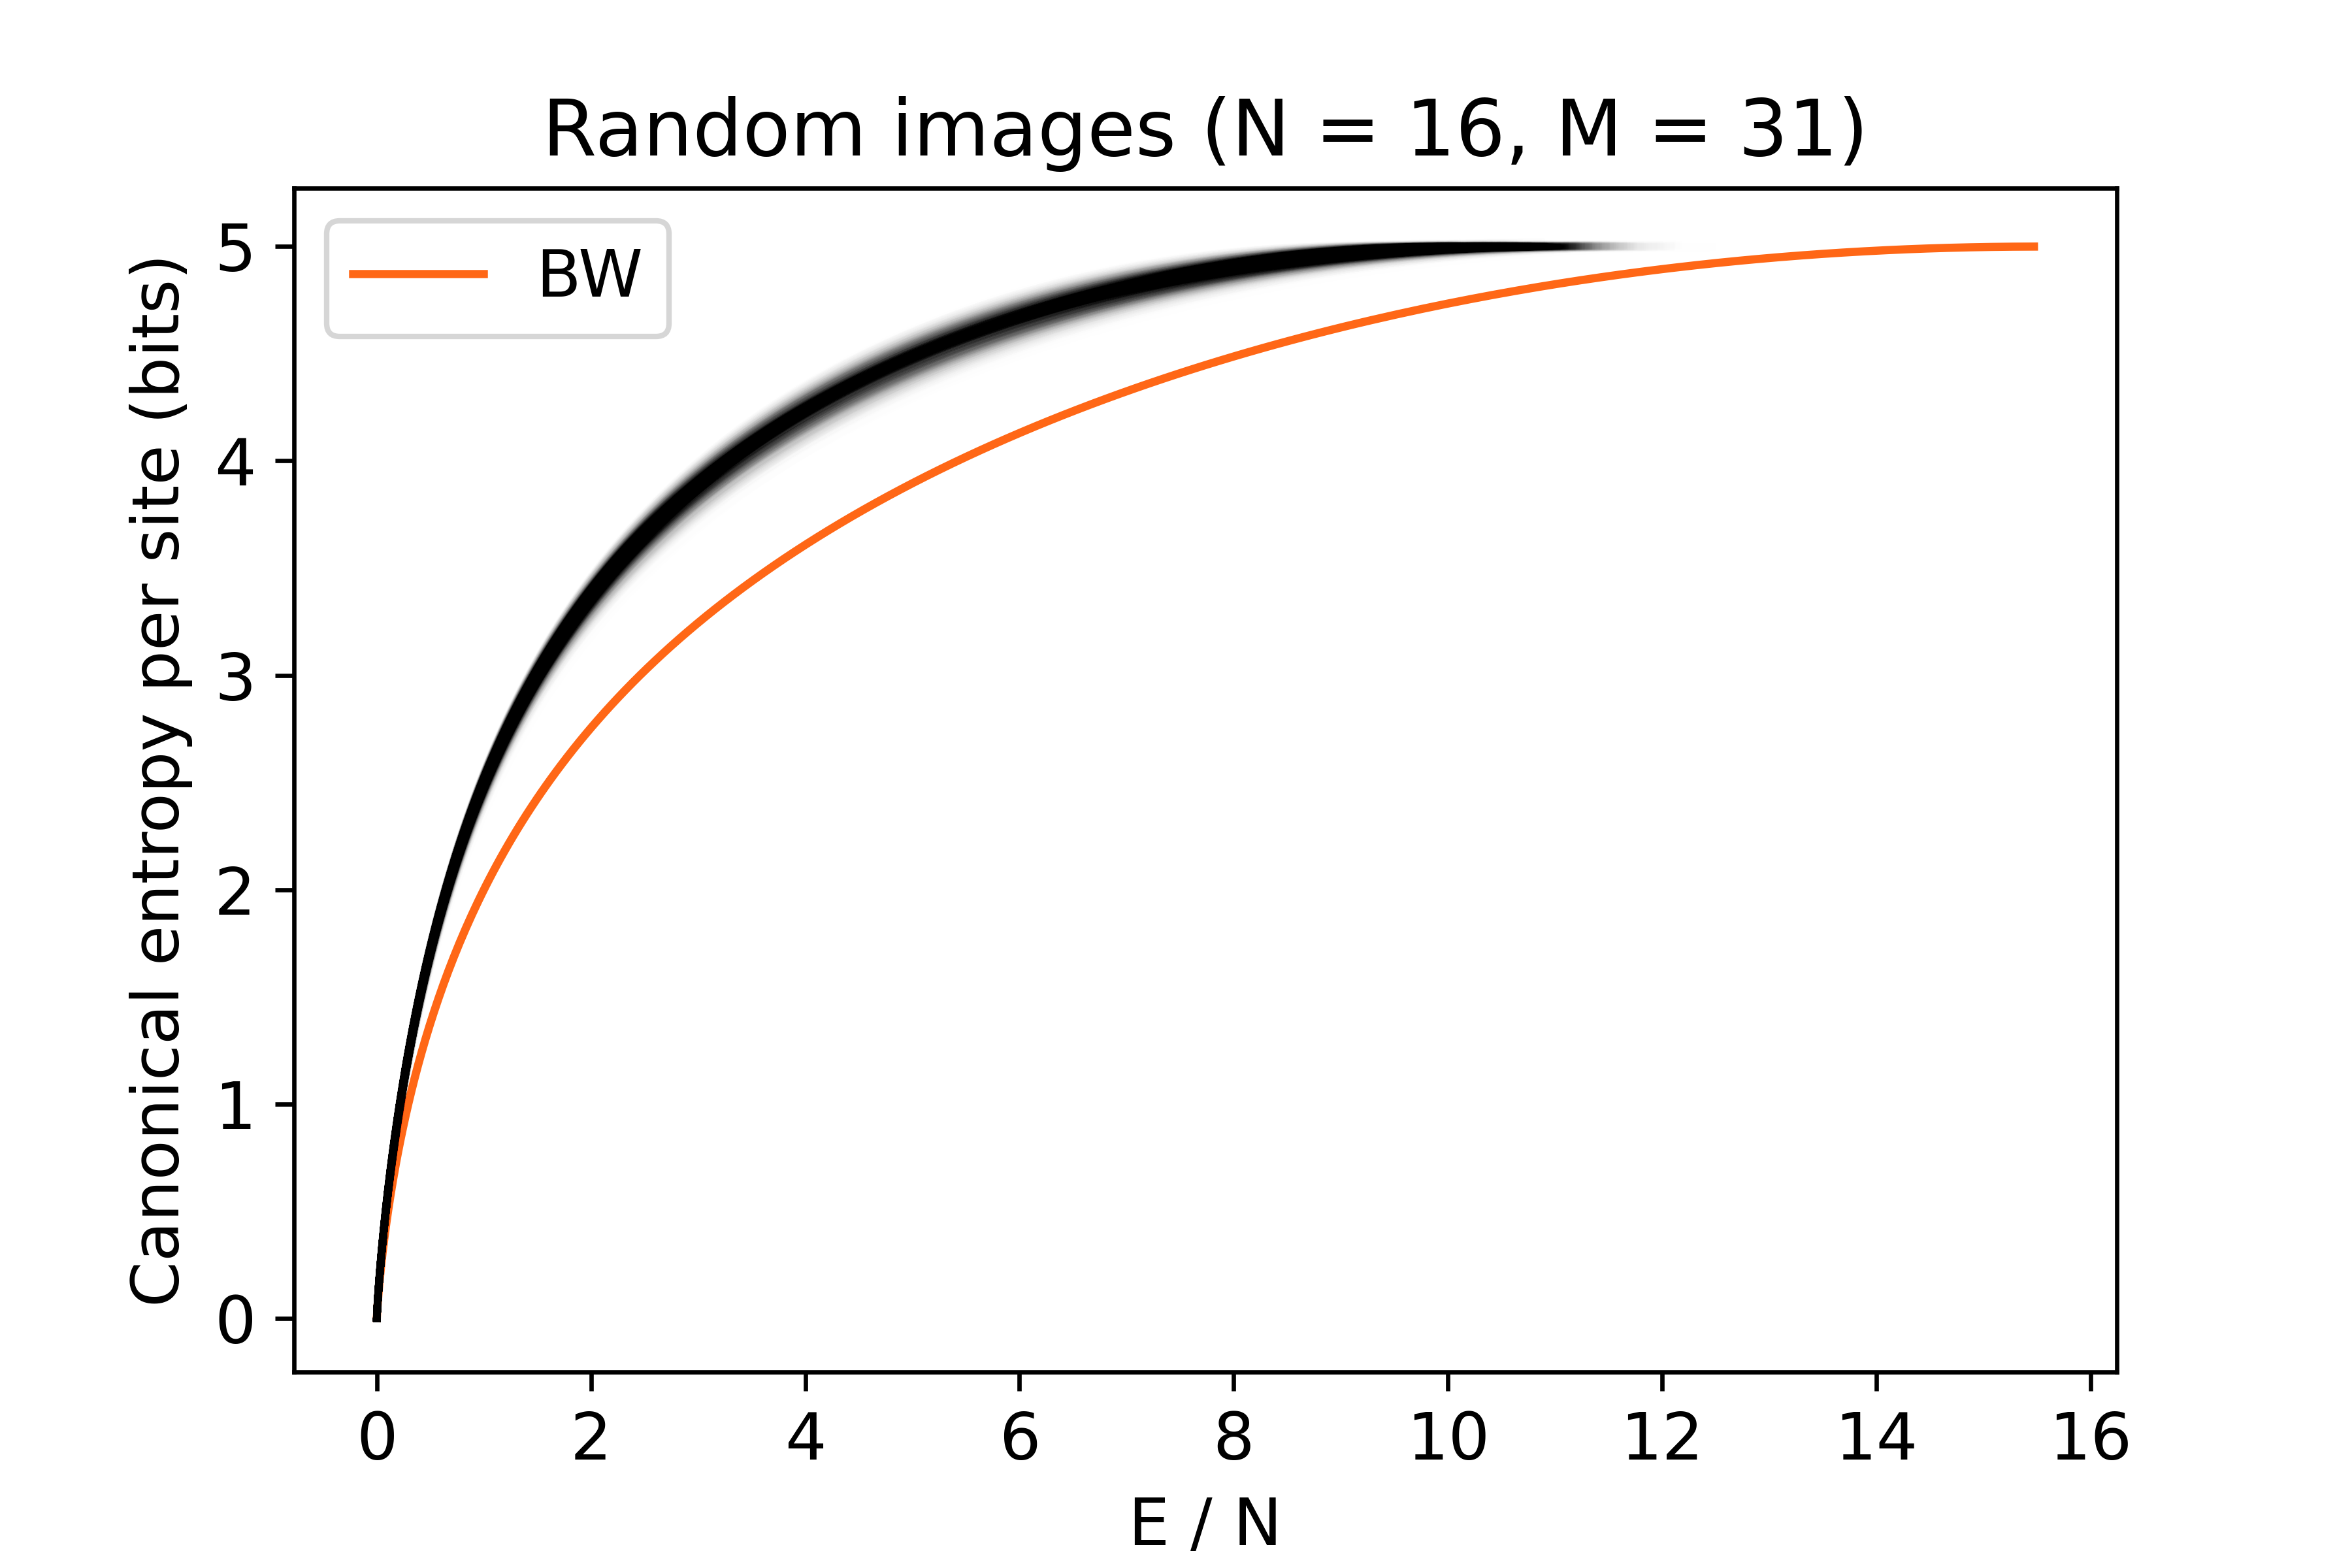
\includegraphics[width=\linewidth]{wanglandau-gray-ES}
  \caption{The canonical entropy for grayscale images increases quickly with
    energy before saturating at the maximum. The entropy from the exact result
  for a black image is shown in orange (BW).}\label{fig:wl-gray-ES}
\end{figure}

The log density of states from WL for a black image is given in
Fig.~\ref{fig:wl-bw}. Since this is indistinguishable from the exact result, we
quantify the error by running \num{1024} simulations for a black image with the
same parameters for histogram flatness and $f$ tolerance as
in~\cite{wanglandau-ajp}. The resulting relative errors are given in
Fig.~\ref{fig:wl-bw-relerror}. This relative error is consistent with that
in~\cite{wanglandau-ajp} for a similarly-sized 2D Ising ferromagnet, which
establishes that the implementation of the algorithm is correct and has the
expected error characteristics.

We now consider the desired calculation of the entropy for random grayscale
images. The WL densities of states for \num{1024} random grayscale images is
given in Fig.~\ref{fig:wl-gray}. The corresponding entropies
(Fig.~\ref{fig:wl-gray-S}) represent the lost information that we seek. The
entropies for different grayscale images are similar, since the local energy
landscapes for gray pixels are close to the same. The entropy for a black image
is lower than for a grayscale image by almost \SI{1}{bit}, which reflects that
the black pixel values may only flucuate up in value, rather than in both
directions for a gray pixel value. We may also see how the entropy depends upon
the average energy, which is the quantity we originally considered
(Fig.~\ref{fig:wl-gray-ES}).

\section{Discussion}

Now that we have computed the lost information as the entropy of a fluctuating
grayscale image, what can we learn from it? The immediate answer is nothing,
since an emperical determination of the average energy $E$ where the difference
between images is barely noticable is required. However, given such a
perscription, we may regard our results as an approximation to the information
lost in visual perception.

The greatest limitation of this approximation is of course the use of a digital
image instead of considering the light impinging on the retina. The pixels in an
image may be considered as averages of the true continuous intensity over a
small solid angle. However, considering a static grid of pixels in a digital
image differs from our foveated imaging process, which features multiple
saccades around a scene to refine points of interest.

Another issue is the arbitrary number of values $M$ for the number of gray
values, which effects the entropy value. The simplest solution is to instead
consider the intensive quantity $\flatfrac{S}{\lg M}$, but it is unclear how to
best generalize this to the case of color, where discretizations of different
colorspaces may produce different results.

Despite these issues, the model of fluctuating pixel values serves as a simple
idealized system that is computationally tractable. This allows us to precisely
specify the problem at hand and begin to work towards a solution.

\section{Conclusion}

TODO.

\appendix

\section{Theorems}

\begin{thm}\label{thm:self-information}
  The only twice continuously differentiable function $I(x)$ that satisfies the
  axioms in Sec.~\ref{sec:information-theory} is the self-information $I(x) =
  -\log p(x)$.
  \begin{proof}
    Consider independent events $x$ and $y$ with probabilities $p$ and $p'$. The
    axioms only concern the probabilities of the events, so we may express the
    information as $I(x) = \tilde{I}(p(x))$. Then as proposed,
    \[
      I(x,\, y)
      = \tilde{I}(pp')
      = \tilde{I}(p) + \tilde{I}(p')
    \]
    by independence. Taking the partial derivative with respect to $p$ gives
    \[
      p' \tilde{I}'(pp')
      = \tilde{I}'(p),
    \]
    and then taking the partial derivative with respect to $p'$ gives
    \[
      \tilde{I}'(pp') + pp' \tilde{I}''(pp')
      = 0.
    \]
    We may then define $q = pp'$ to obtain the differential equation
    \[
      \dv{q}\qty(q \tilde{I}'(q))
      = 0,
    \]
    which has solution
    \[
      \tilde{I}(q) = k\log q
    \]
    for real $k$. The condition that $\tilde{I}(q) \ge 0$ requires $k > 0$,
    which is equivalent to a choice of base for the logarithm.
  \end{proof}
\end{thm}

\begin{thm}\label{thm:bw-g}
  The number of tuples $(a_1,\, \ldots,\, a_N)$ with $0 \leq a_i \leq M - 1$ and
  $\sum_i a_i = E$ is
  \[
    g(E)
    = \sum_k {(-1)}^k \binom{N}{k} \binom{N + E - Mk - 1}{E - Mk}.
  \]
  \begin{proof}
    We represent the sum $E$ as the exponent of a integer polynomial in $z$ in
    the following way. For the tuple $(x_1,\, x_2)$, we represent $x_1$ as
    $z^{x_1}$ and $x_2$ as $z^{x_2}$. Together, we have $z^{x_1} z^{x_2}$,
    which gives the monomial $z^{x_1 + x_2} = z^E$ for this tuple. We may then
    find $g(E)$ as the coefficient of $z^E$ in
    \[
      {\qty(1 + \cdots + z^{M-1})}^N.
    \]
    Expanding using the binomial theorem gives
    \begin{align}
      {\qty(\frac{1 - z^M}{1 - z})}^N
      &= \sum_{k=0}^N {(-1)}^k \binom{N}{k} z^{Mk}
      \sum_{j=0}^\infty {(-1)}^j \binom{-N}{j} z^j \\
      &= \sum_{k=0}^N \sum_{j=0}^\infty {(-1)}^k \binom{N}{k}
      \binom{N + j - 1}{j} z^{Mk + j}.
    \end{align}
    The value of $j$ for $z$ to have exponent $E$ is $j = E - Mk$, so the
    coefficient of $z^E$ in the polynomial is
    \begin{equation}
      g(E)
      = \sum_k {(-1)}^k \binom{N}{k} \binom{N + E - Mk - 1}{E - Mk},
    \end{equation}
    where the limits of summation are set by the binomial coefficients.
  \end{proof}
\end{thm}

\section{Wang-Landau algorithm implementation}\label{sec:wanglandau-core}

The relevant core of the Wang-Landau algorithm implementation is reproduced
below. For the full code, see the \textsc{reu} project
repository~\cite{rpi-reu-notebook}.

\inputminted{python}{wanglandau-core.py}

\nocite{*}
\hypersetup{urlcolor=Mahogany}
\bibliography{references}

\end{document}

